\section{Implementierung}


\subsection{Design}
\begin{frame} %%Eine Folie
  \frametitle{Design} %%Folientitel
% Definitionsblock
  \begin{block}{Anforderungen and das Design:}

	 \begin{itemize}
    	\begin{multicols}{2}
	\item drei Spaltenlayout
	\item Box-Shadow
	\item Textshadow
	\item Borderradius
	\item Font einbinden
	\item ...
    \end{multicols}
  \end{itemize}
  \end{block}

% Definitionsblock
  \begin{block}{Motivation:}

Intuitiv und übersichtliches Design unter Berücksichtigung der Vorgaben
  \end{block}

  \begin{block}{Idee:}

Gliederung der Inhalte in Boxen
  \end{block}

\end{frame}


\defverbatim[colored]
  \makeset{
    \jscode

      \begin{lstlisting}[name=cssmenu.css]			

.basic-wrapper{
    background-color: #ffffff;
    padding:10px;
    margin: 0px 10px 15px;
    border: solid 1px #c3c5c9;
    -webkit-border-radius: 4px;
    -moz-border-radius: 4px;
    border-radius: 4px;
}

.basic-wrapper-top{
    background-color:#DE8642;
    text-align:center;
    font-family: 'Changa One', cursive;
    font-size:120%;
    text-transform: uppercase;
    margin: 0px 10px;
    padding:3px;
    overflow:hidden;
    border: solid 1px #c3c5c9;
    -webkit-border-top-left-radius: 4px;
    -webkit-border-top-right-radius: 4px;
    -moz-border-radius-topleft: 4px;
    -moz-border-radius-topright: 4px;
    border-top-left-radius: 4px;
    border-top-right-radius: 4px;
}

      \end{lstlisting}
  }


\begin{frame}
  \frametitle{Umsetzung der Design-Idee}
  \makeset
\end{frame}


\defverbatim[colored]
  \makeset{
    \jscode

      \begin{lstlisting}[name=cssmenu.css]			

.basic-wrapper-middle{
    background-color: #ffffff;
    padding:0 10px;
    overflow:hidden;
    border-left: solid 1px #c3c5c9;
    border-right: solid 1px #c3c5c9;
    margin: 0px 10px auto;
}
.basic-wrapper-bottom{
    background-color: #ffffff;
    padding:10px 10px 10px 10px;
    overflow:hidden;
    margin: 0px 10px 15px;
    border-left: solid 1px #c3c5c9;
    border-right: solid 1px #c3c5c9;
    border-bottom: solid 1px #c3c5c9;
    -webkit-border-bottom-right-radius: 4px;
    -webkit-border-bottom-left-radius: 4px;
    -moz-border-radius-bottomright: 4px;
    -moz-border-radius-bottomleft: 4px;
    border-bottom-right-radius: 4px;
    border-bottom-left-radius: 4px;
}
      \end{lstlisting}
  }


\begin{frame}
  \frametitle{Umsetzung der Design-Idee}
  \makeset
\end{frame}


\begin{frame}

\begin{figure}[!htbp]
 \centering
\frametitle{Umsetzung der Design-Idee}
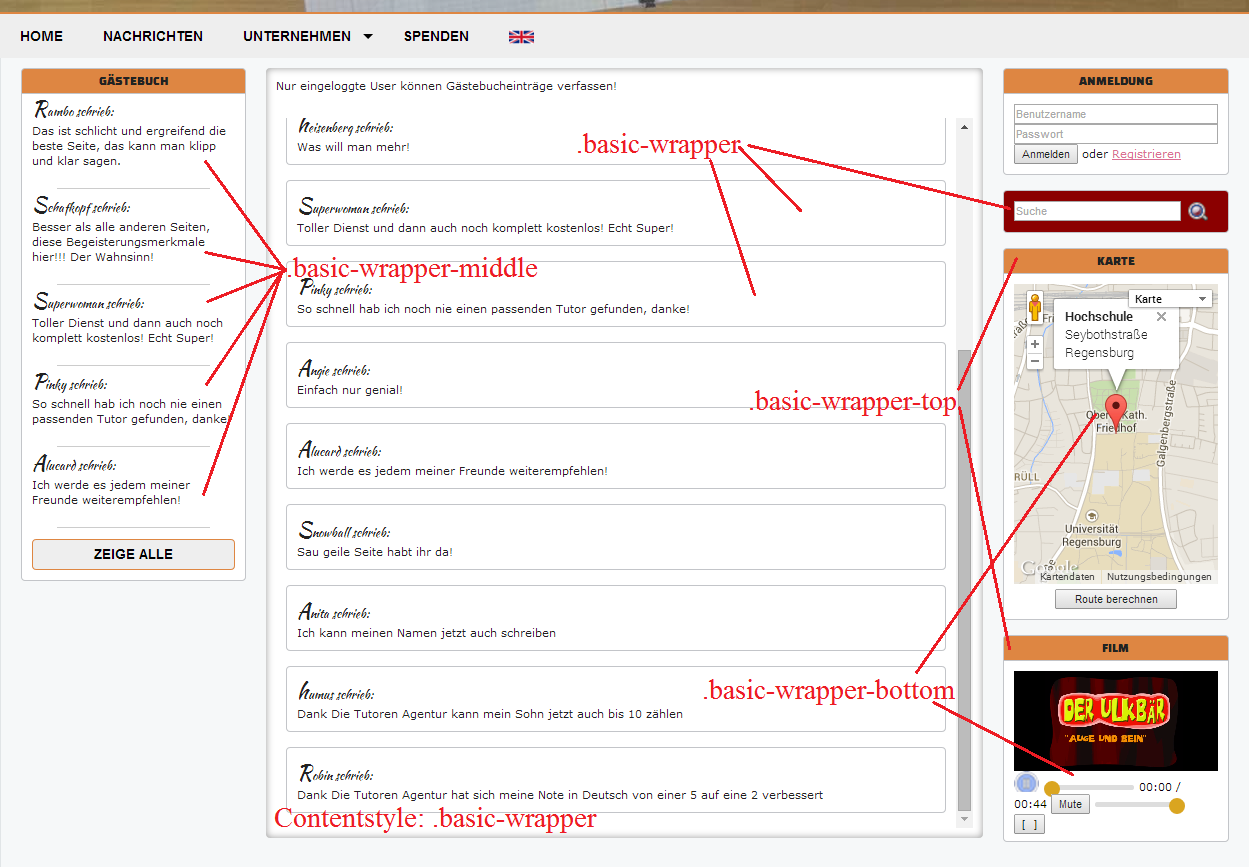
\includegraphics[width=0.9\linewidth]{./Source/Screenwrapper.png}
 \caption{Screenshot Design}
\end{figure}

\end{frame}


\defverbatim[colored]
  \makeset{
    \jscode

      \begin{lstlisting}[name=boxshadow.css]			
.boxshadow #content
{
    -webkit-box-shadow: inset 0px 0px 10px 0px rgba(0, 0, 0, 0.4); /* WebKit */
    -moz-box-shadow: inset 0px 0px 10px 0px rgba(0, 0, 0, 0.4); /* Firefox */
    box-shadow: inset 0px 0px 10px 0px rgba(0, 0, 0, 0.4); /* Standard */
    border:0;
}

h2
{
    font-size:20px;
    font-weight: normal;
    margin:0;
    text-shadow: #c0c0c0 3px 3px 5px;
}
.lt-ie9 h2
{
	/* For IE 8 */
	-ms-filter: "progid:DXImageTransform.Microsoft.Shadow(Strength=2, Direction=135, Color='#000000')";
	/* For IE 5.5 - 7 */
	filter: progid:DXImageTransform.Microsoft.Shadow(Strength=2, Direction=135, Color='#000000');	
}



      \end{lstlisting}
  }

\begin{frame}
  \frametitle{Boxshadow, Textshadow, Font}
  \makeset
\end{frame}


\defverbatim[colored]
  \makeset{
    \phpcode

      \begin{lstlisting}[name=font.php]			
 <!-- font -->
        <link href='http://fonts.googleapis.com/css?family=Yesteryear' rel='stylesheet' type='text/css'>
        <link href='http://fonts.googleapis.com/css?family=Berkshire+Swash' rel='stylesheet' type='text/css'>
        <link href='http://fonts.googleapis.com/css?family=Changa+One' rel='stylesheet' type='text/css'>
        <link href='http://fonts.googleapis.com/css?family=Lobster' rel='stylesheet' type='text/css'>
        <link href='http://fonts.googleapis.com/css?family=Kaushan+Script' rel='stylesheet' type='text/css'>

      \end{lstlisting}
  }

\begin{frame}
  \frametitle{Boxshadow, Textshadow, Font}
  \makeset
\end{frame}

\begin{frame}

\frametitle{Boxshadow, Textshadow, Font}
\begin{figure}[!htbp]
 \centering
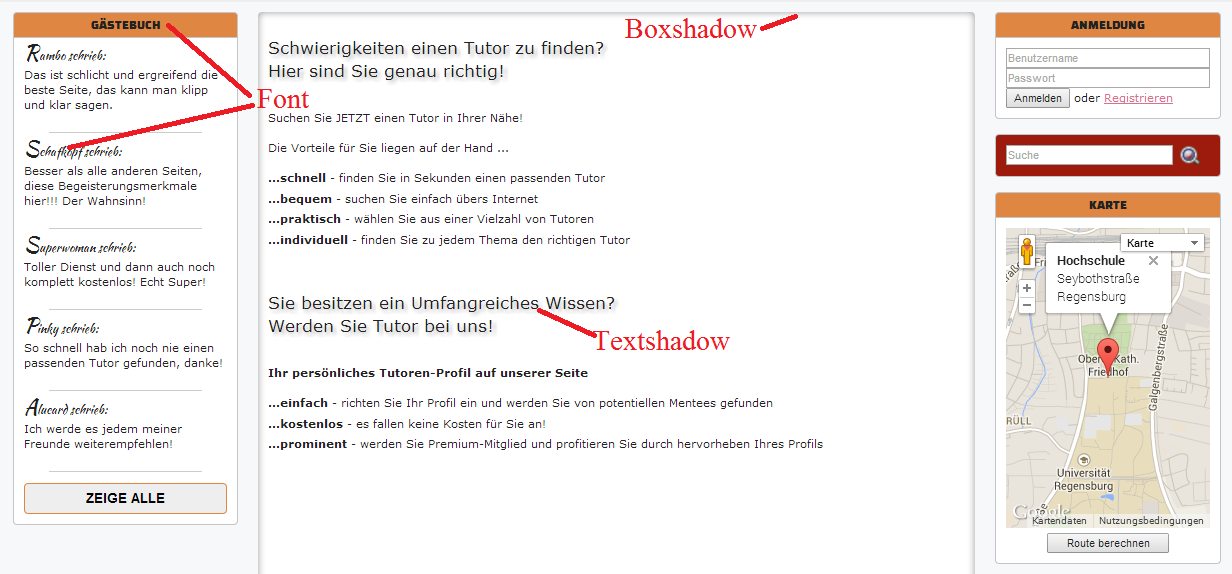
\includegraphics[width=0.9\linewidth]{./Source/boxshadow.png}
 \caption{Screenshot zum Box-und Textshadow}

\end{figure}

\end{frame}

\begin{frame}

\frametitle{Boxshadow, Textshadow, Font}
\begin{figure}[!htbp]
 \centering

\includegraphics[width=0.9\linewidth]{./Source/IE8textshadow.png}
 \caption{Screenshot zum Box-und Textshadow IE8}

\end{figure}

\end{frame}



\subsection{Menü}

\begin{frame} %%Eine Folie
  \frametitle{Menü} %%Folientitel


% Definitionsblock
  \begin{block}{Anforderung:}
	"Die Navigation soll über ein Menü erfolgen. Auch ein Top-Down-Menü soll realisiert werden."
  \end{block}

  \begin{block}{Motivation:}
	"Das Menü soll so implementiert werden, dass jederzeit neue Menüpunkte hinzugefügt werden können oder entfernt werden können"
  \end{block}
\end{frame}


\defverbatim[colored]
  \makeset{
    \phpcode

      \begin{lstlisting}[name=menu.php]			
				<ul>
					<li><a href="/en/index.php"><span>Home</span></a></li>
					<li><a href="/en/news.php"><span>News</span></a></li>
					<li class="has-sub"><a><span>Corporate</span></a>
						<ul>
                            <li><a href="/en/corporate.php"><span>The Tutoren AG</span></a>
							<li><a href="/en/contact.php"><span>Contact</span></a></li>
							<li class="last"><a href="/en/guestbook.php"><span>Guestbook</span></a></li>
						</ul>
					</li>
					<li><a href="/en/donate.php"><span>Donation</span></a></li>
                    <?php
                        if ( $_SESSION['admin'] == true )
                        {
                            echo '<li><a href="/private/index.php"><span>Private folder</span></a></li>';
                        }
                        if ( $_SESSION['logged-in'] == true )
                        {
                            echo '<li><a href="/en/profile.php"><span>Profile</span></a></li>';
                        }
                    ?>
					<li><?php echo '<a href="/de/'.$forwardto.'"><img src="/images/de.png" class="flag_img" alt="DE-Flagge"></a>'; ?> </li>		
				</ul>
		<?php
      \end{lstlisting}
  }


\begin{frame}
  \frametitle{Html-Liste für das Menü}
  \makeset
\end{frame}


\defverbatim[colored]
  \makeset{
    \jscode

      \begin{lstlisting}[name=cssmenu.css]			

.cssmenu > ul 
{
	position: relative;
	display: block;
	background: #EEEEEE;
	height: 32px;
	width: 100%;
	z-index:10;
}

.cssmenu ul ul 
{
  position: absolute;
  top: 70px;
  opacity: 0;
  left: -99999px;
  /*for a better look in browser that support the cssanimations*/
  -webkit-transition: opacity .3s ease, top .25s ease;
  -moz-transition: opacity .3s ease, top .25s ease;
  -ms-transition: opacity .3s ease, top .25s ease;
  -o-transition: opacity .3s ease, top .25s ease;
  transition: opacity .3s ease, top .25s ease;
  z-index: -99;
}

      \end{lstlisting}
  }

\begin{frame}
  \frametitle{CSS-Implementierung für das Menü}
  \makeset
\end{frame}


\defverbatim[colored]
  \makeset{
    \jscode

      \begin{lstlisting}[name=cssmenu.css]			

.cssmenu ul > li:hover > ul 
{
  left: auto;
  top: 44px;
  opacity: 1;
}

.cssmenu ul ul li:hover > ul 
{
  left: 170px;
  top: 0;
  opacity: 1;
}


}

      \end{lstlisting}
  }


\begin{frame}
  \frametitle{CSS-Implementierung für das Menü}
  \makeset
\end{frame}






\subsection{Responsive Webdesign}
\begin{frame} %%Eine Folie
  \frametitle{Responsive Webdesign} %%Folientitel
% Definitionsblock
  \begin{block}{Anforderung:}
  Für die Webseite soll ein responsives Webdesign implementiert werden, so dass sie auf verschiedenen Geräten
  mit unterschiedlichen Aufklösungen dargestellt werden kann.
  \end{block}


% Definitionsblock
  \begin{block}{Realisierung:}
	 \begin{itemize}

	\item Prozentuale Größen für Breiten
	\item ... aber maximale Gesamtbreite 1250px
	\item Höhenanpassung für Slideshow und Logo über Css-Media-Queries
	\item Neuanordnung der der Spalten für kleine Auflösungen
\end{itemize}

  \end{block}

\end{frame}


\defverbatim[colored]
  \makeset{
    \jscode
      \begin{lstlisting}[name=responsive.php]			

@media screen and (max-width: 400px)
{
    #wrapper{
        min-height:2245px;
        height:auto;
    }
    #content{
		width:92.8%;
		margin: 0 1.6%;
		margin-top:10px;
	}
    #left{

        top:1575px;
        float:left;
        width:100%;
        margin-bottom: 1.6%;;
    }
    #right{
        float:left;
        width:100%;
        margin-bottom: 1.6%;
    }
    #banner {
        height:100px;
  }

      \end{lstlisting}
  }

\begin{frame}
  \frametitle{Responsive Webdesign}
  \makeset
\end{frame}

\defverbatim[colored]
  \makeset{
    \jscode
      \begin{lstlisting}[name=responsive.php]			
    #show {
        width:100%; 
        height:100px;
    }
    .slider_img {
        width:100%;
        height:100px;
    }
    .logo_img{
        width:100px; 
        min-height:100px;
		height:100%;
	}
}

      \end{lstlisting}
  }

\begin{frame}
  \frametitle{Responsive Webdesign}
  \makeset
\end{frame}

\begin{frame}
  \frametitle{Responsive Webdesign}
\begin{figure}[!htbp]
 \centering
 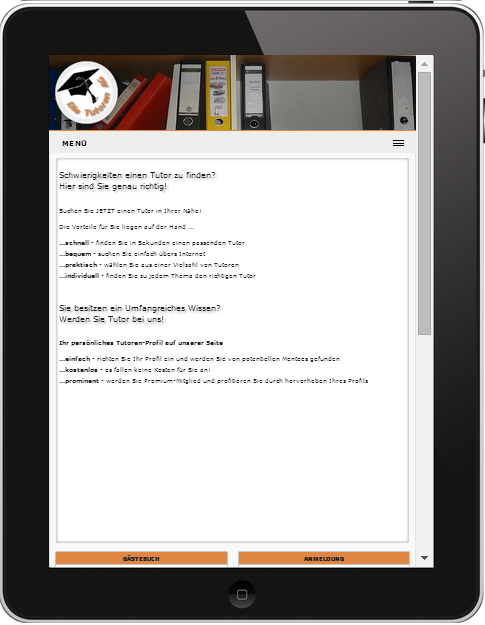
\includegraphics[scale=.3]{./Source/Ipad.png}
 \caption{iPad erstellt mit www.http://deviceponsive.com/}

\end{figure}
\end{frame}

\begin{frame}
  \frametitle{Responsive Webdesign}
\begin{figure}[!htbp]
 \centering
 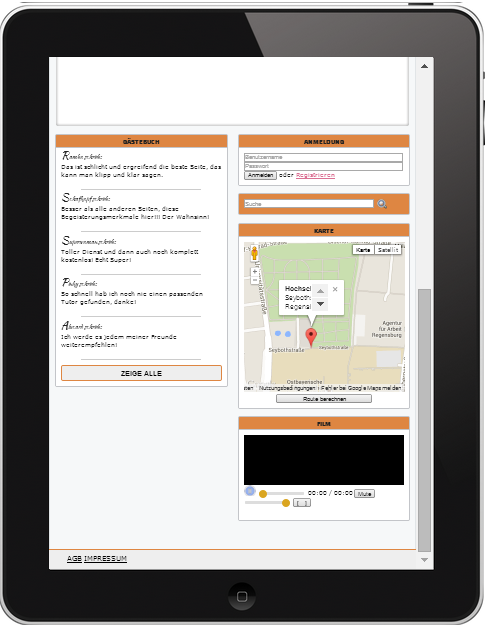
\includegraphics[scale=.3]{./Source/Ipad2.png}
 \caption{iPad erstellt mit www.http://deviceponsive.com/}

\end{figure}
\end{frame}

\begin{frame}
  \frametitle{Responsive Webdesign}
\begin{figure}[!htbp]
 \centering
 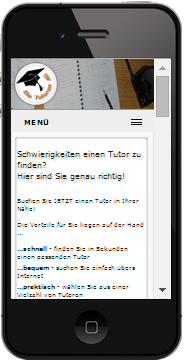
\includegraphics[scale=0.5]{./Source/Iphone1.png}
 \caption{iPhone erstellt mit www.http://deviceponsive.com/}

\end{figure}
\end{frame}

\begin{frame}
  \frametitle{Responsive Webdesign}
\begin{figure}[!htbp]
 \centering
 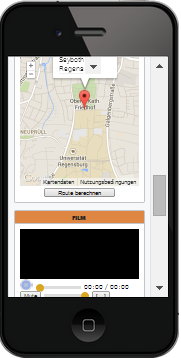
\includegraphics[scale=0.5]{./Source/Iphone2.png}
 \caption{iPhone erstellt mit www.http://deviceponsive.com/}

\end{figure}
\end{frame}

\subsection{Testphase}
\begin{frame} %%Eine Folie
\frametitle{Testphase} %%Folientitel
  \textbf{Design auf Cross-Kompatibilität getestet: }
% Definitionsblock
  \begin{block}{Realisierung:}
	 \begin{itemize}

	\item unterschiedlichen Browsern und Versionen
	\item Developer Toolbars
	\item http://www.browserstack.com/
	\item http://browsershots.org/
 \end{itemize}
\end{block}


\end{frame}







\subsection{Demonstration}
\begin{frame} %%Eine Folie
  \frametitle{Demonstration} %%Folientitel

% Fettgedruckt
  \center
  \textbf{Es folgt eine Demonstration ...}
\end{frame}